\documentclass[xcolor=table,aspectratio=169]{beamer}
\usepackage{beamerthemesplit}
\usepackage{wrapfig}
\usetheme{SPbGU}
\usepackage{pdfpages}
\usepackage{amsmath}
\usepackage{cmap}
\usepackage[T2A]{fontenc}
\usepackage[utf8]{inputenc}
\usepackage[english]{babel}
\usepackage{indentfirst}
\usepackage{mathtools}
\usepackage{tikz}
\usepackage{multirow}
\usepackage[noend]{algpseudocode}
\usepackage{algorithm}
\usepackage{algorithmicx}
\usepackage{fancyvrb}

\usepackage{minted}

\usetikzlibrary{calc}
\usetikzlibrary{shapes,arrows}
\usetikzlibrary{arrows,automata}
\usetikzlibrary{positioning}

\usepackage{fontawesome}

\usetikzlibrary{shapes.callouts}

\usepackage{xparse}

%for [[ ]]
\usepackage{stmaryrd}


\tikzset{
    invisible/.style={opacity=0,text opacity=0},
    visible on/.style={alt=#1{}{invisible}},
    alt/.code args={<#1>#2#3}{%
      \alt<#1>{\pgfkeysalso{#2}}{\pgfkeysalso{#3}} % \pgfkeysalso doesn't change the path
    },
}

\NewDocumentCommand{\mycallout}{r<> O{opacity=0.8,text opacity=1} m m}{%
\tikz[remember picture, overlay]\node[align=center, fill=cyan!20, text width=3.5cm,
#2,visible on=<#1>, rounded corners,
draw,rectangle callout,anchor=pointer,callout relative pointer={(230:1cm)}]
at (#3) {#4};
}

%\newcommand{\tikzmark}[1]{\tikz[overlay,remember picture,baseline=-0.5ex] \node (#1) {};}



\usepackage{tabularx}
\newcolumntype{Y}{>{\raggedleft\arraybackslash}X}

\renewcommand{\thealgorithm}{}

\newtheorem{mytheorem}{Theorem}
\renewcommand{\thealgorithm}{}

\newcommand{\tikzmark}[1]{\tikz[overlay,remember picture] \node (#1) {};}
\def\Put(#1,#2)#3{\leavevmode\makebox(0,0){\put(#1,#2){#3}}}

\newcommand{\ltz}{$< 1$}


\tikzset{
    state/.style={
           rectangle,
           rounded corners,
           draw=black, very thick,
           minimum height=2em,
           inner sep=2pt,
           text centered,
           },
}

\beamertemplatenavigationsymbolsempty

\title[Multiple-Source CFPQ]{Multiple-Source Context-Free Path Querying in Terms of Linear Algebra}
%\subtitle[YaccConstructor]{Parsing techniques for graph analysis}
\institute[JB Research, SPbSU]{
JetBrains Research, Programming Languages and Tools Lab  \\
Saint Petersburg University
}


\author[Semyon Grigorev]{Arseniy Terekhov, Vlada Pogozhelskaya, Vadim Abzalov, Timur Zinnatulin, \textbf{Semyon Grigorev}}

\date{March 24, 2021}

\begin{document}
{
\begin{frame}[fragile]
  \begin{table}
  \centering
  \begin{tabularx}{\linewidth}{XcX}
    
\includegraphics[height=1.5cm]{pictures/JB_logo_RGB_research_vert.pdf} \hfill
    & \begin{minipage}[t]{0.3\textwidth}\center 
\includegraphics[height=1.5cm]{pictures/EDBT.png} \hfill
      \end{minipage}
    & \hfill 
\includegraphics[height=1.5cm]{pictures/SPbGU_Logo.png}
  \end{tabularx}
  \end{table}
  \titlepage
\end{frame}
}

\begin{frame}[fragile] \frametitle{Formal Language Constrained Path Querying}
      \begin{minipage}[m]{0.45\linewidth}
  \raisebox{-0.5\totalheight}{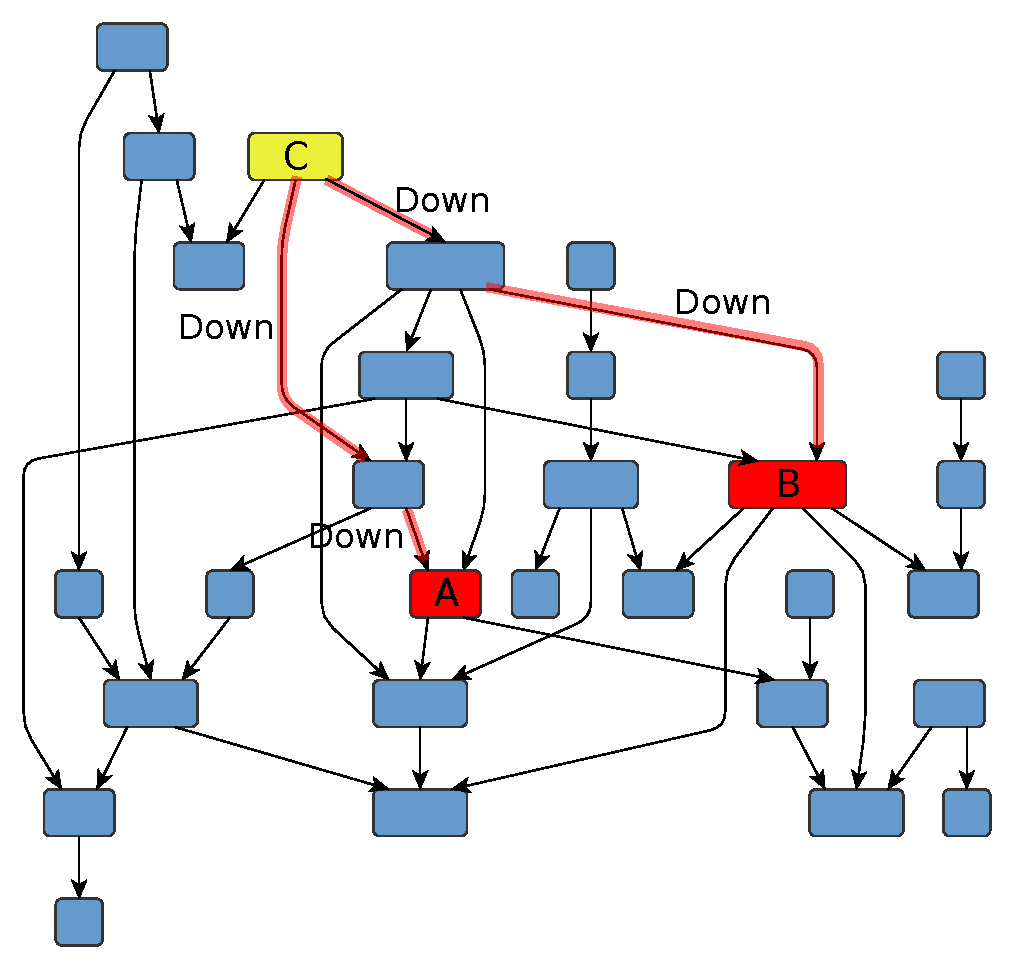
\includegraphics[width=\textwidth]{pictures/hierarchical.pdf}}
  \end{minipage}\hfill
  \begin{minipage}[m]{0.5\linewidth}
  Navigation through a graph
  \begin{itemize}
        \item Are nodes A and B on the same level of hierarchy?
        \item Is there a path of form $\textbf{Up}^n \, \textbf{Down}^n$?
        \item Find all paths of form $\textbf{Up}^n \, \textbf{Down}^n$ which start from the~node A
  \end{itemize}

  \end{minipage}

  \end{frame}

\begin{frame}[fragile] \frametitle{Context-Free Path Querying (CFPQ)}
   \begin{itemize}
    \item Applications
    \begin{itemize}
      \item Static code analysis
      \item Graph segmentation
    \end{itemize}
    \item Theory
    \begin{itemize}
      \item !!!
      \item !!!
    \end{itemize}
    \pause
    \item Integration with real-world systems
    \begin{itemize}
      \item !!!!
      \item Kuijpers for Neo4j: too slow to be practical
      \pause
      \item RedisGraph
    \end{itemize}

  \end{itemize}
\end{frame}

\begin{frame}[fragile] \frametitle{Linear Algebra Based CFPQ Algorithm}
  \begin{itemize}
    \item Definition
    \begin{itemize}
      \item Special DSL which can be specialized and compiled
      \item Ahead-of-time specialization
    \end{itemize}
    \item Impractical memory consumption
    \begin{itemize}
      \item Na\"{\i}ve multiple substring matching
      \item 2D convolution
    \end{itemize}
    \item Context-Free grammars are too hard to be used by end-users
    \begin{itemize}
      \item \textbf{GTX-1070}: Pascal architecture, 8GB GDDR5, 1920 CUDA cores
      \item \textbf{Tesla T4}: Turing architecture, 16GB GDDR6, 2560 CUDA cores
    \end{itemize}

  \end{itemize}
\end{frame}


\begin{frame}[fragile] \frametitle{Proposed Solution}
  \begin{itemize}
      \item RedisGraph
      \item Cypher\footnote{!!!}
      \item Multiple-Soource CFPQ
  \end{itemize}
  \begin{center}
  \begin{minipage}[t]{0.48\textwidth}
    \begin{center}
      \tikzmark{x}{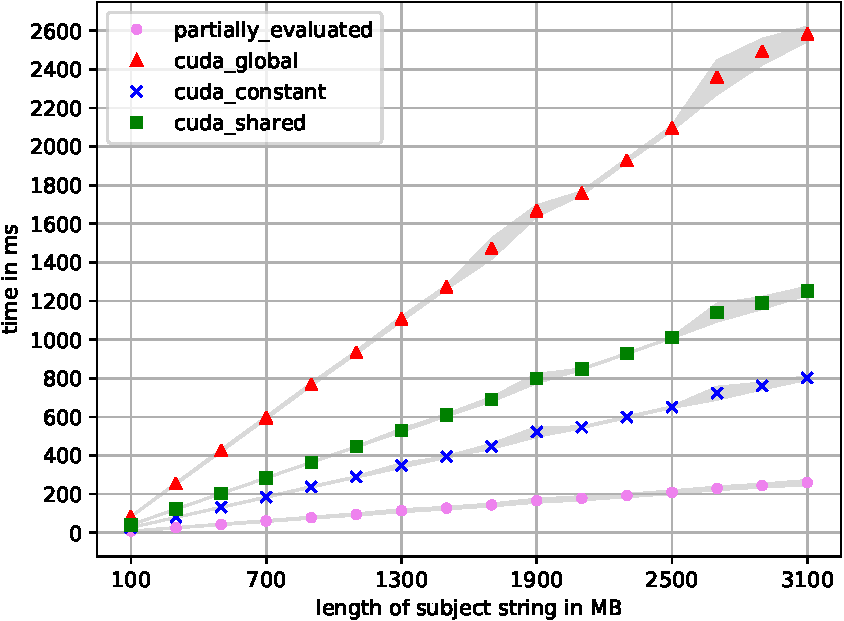
\includegraphics[width=\textwidth]{pictures/Substr_1070-crop}}
  \\Results for GTX-1070
\end{center}
\end{minipage}
\begin{minipage}[t]{0.48\textwidth}
  \begin{center}
{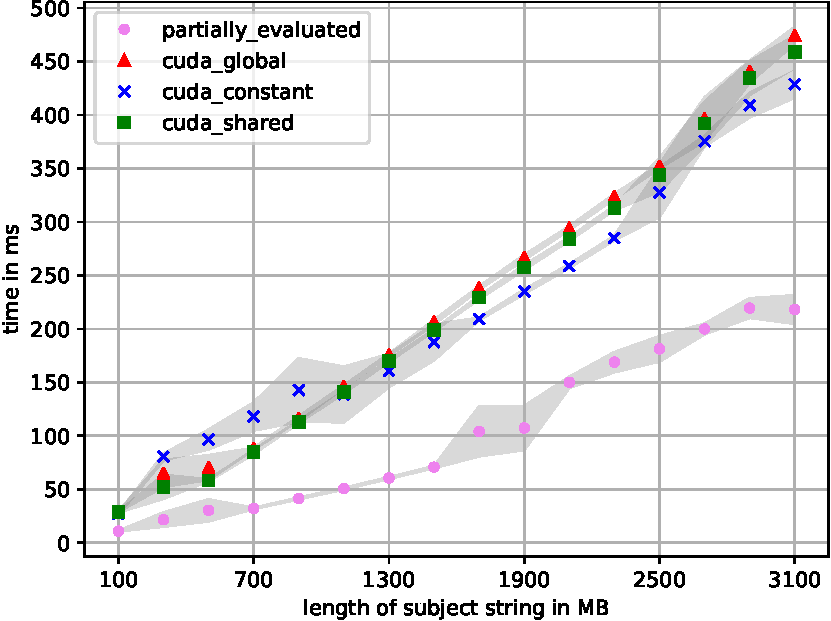
\includegraphics[width=\textwidth]{pictures/Substr_T4-crop}}
\\Results for Tesla T4
\end{center}
\end{minipage}
\end{center}
\end{frame}


\begin{frame}[fragile] \frametitle{Multiple-Source CFPQ}
  \begin{itemize}
  \item Application: image processing
  \item Subject image: random image  of size 1GB %(16384 * 16384)
  \item Filters: random square filters with diameter 3 to 255
  \end{itemize}
  \begin{center}
  \begin{minipage}[t]{0.48\textwidth}
    \begin{center}
  \tikzmark{y}{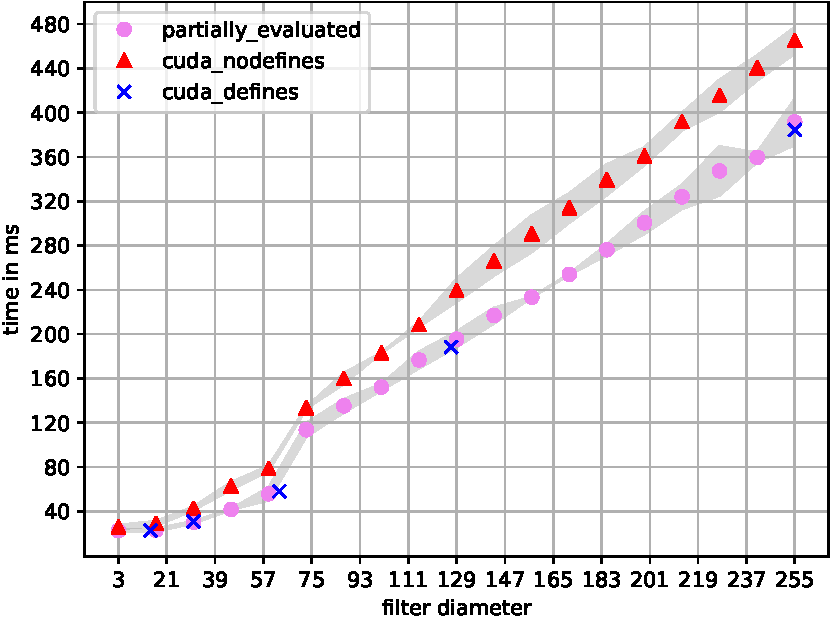
\includegraphics[width=\textwidth]{pictures/Conv_1070-crop}}
  \\Results for GTX-1070
\end{center}
\end{minipage}
\begin{minipage}[t]{0.48\textwidth}
  \begin{center}
{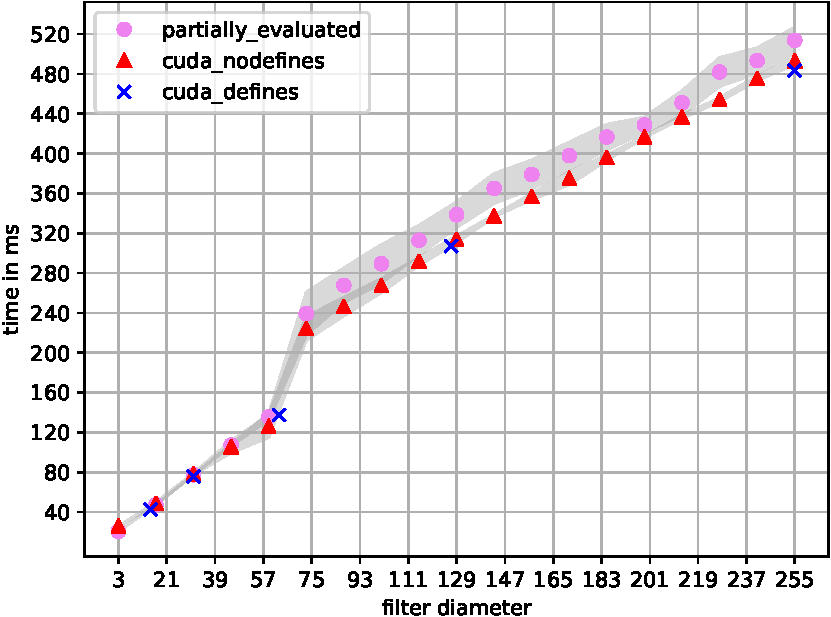
\includegraphics[width=\textwidth]{pictures/Conv_T4-crop}}
\\Results for Tesla T4
\end{center}
\end{minipage}
\end{center}
\end{frame}


\begin{frame}[fragile] \frametitle{Implementation Details}
  \begin{itemize}
  \item Application: image processing
  \item Subject image: random image  of size 1GB %(16384 * 16384)
  \item Filters: random square filters with diameter 3 to 255
  \end{itemize}
  \begin{center}
  \begin{minipage}[t]{0.48\textwidth}
    \begin{center}
  \tikzmark{y}{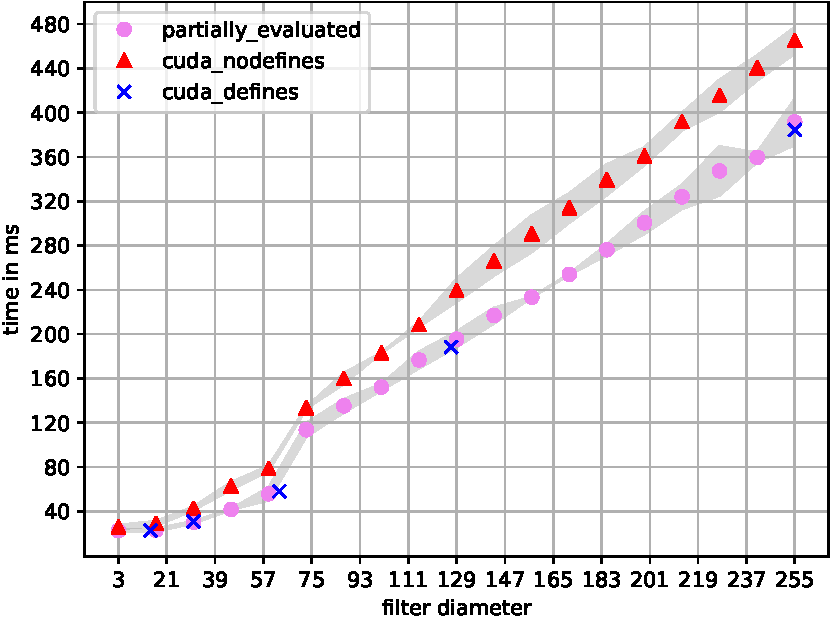
\includegraphics[width=\textwidth]{pictures/Conv_1070-crop}}
  \\Results for GTX-1070
\end{center}
\end{minipage}
\begin{minipage}[t]{0.48\textwidth}
  \begin{center}
{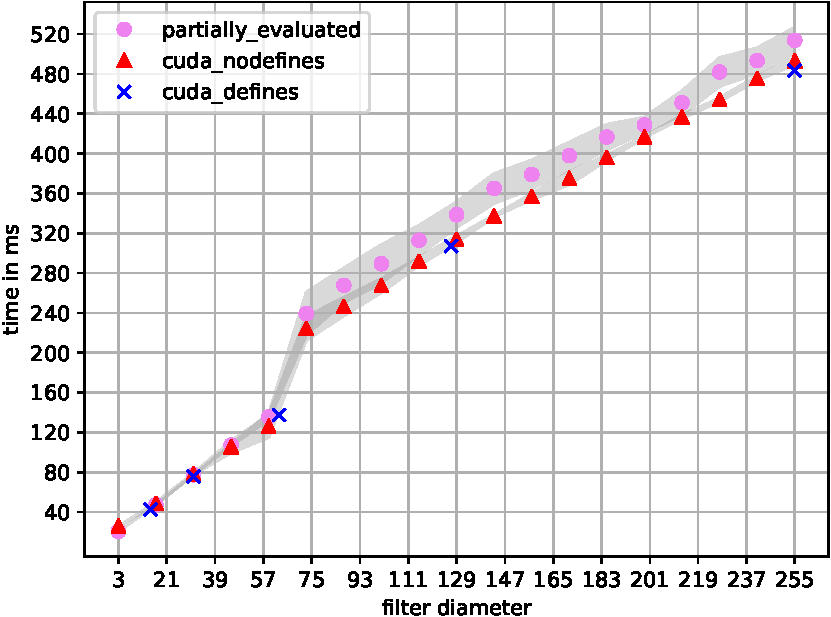
\includegraphics[width=\textwidth]{pictures/Conv_T4-crop}}
\\Results for Tesla T4
\end{center}
\end{minipage}
\end{center}
\end{frame}


\begin{frame}[fragile] \frametitle{Cypher Extension}
  \begin{itemize}
  \item Application: image processing
  \item Subject image: random image  of size 1GB %(16384 * 16384)
  \item Filters: random square filters with diameter 3 to 255
  \end{itemize}
  \begin{center}
  \begin{minipage}[t]{0.48\textwidth}
    \begin{center}
  \tikzmark{y}{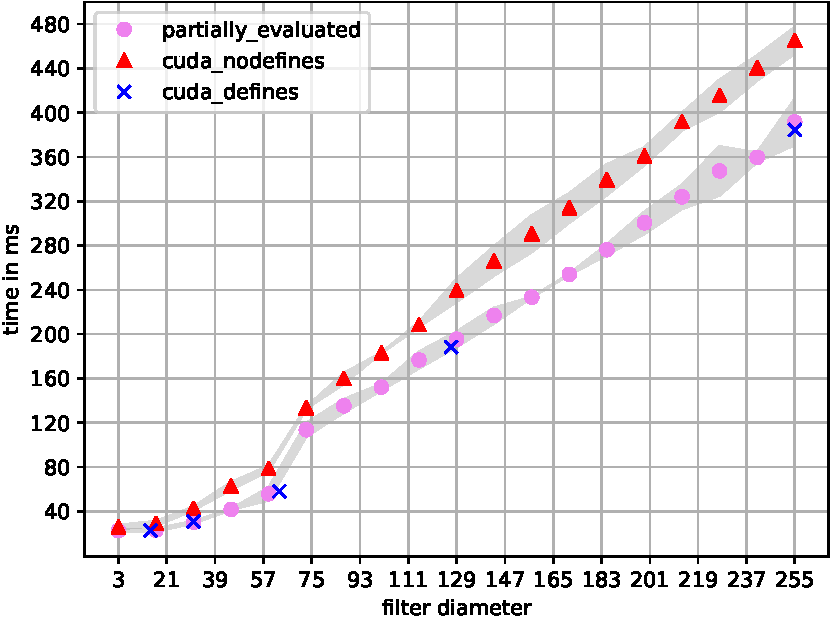
\includegraphics[width=\textwidth]{pictures/Conv_1070-crop}}
  \\Results for GTX-1070
\end{center}
\end{minipage}
\begin{minipage}[t]{0.48\textwidth}
  \begin{center}
{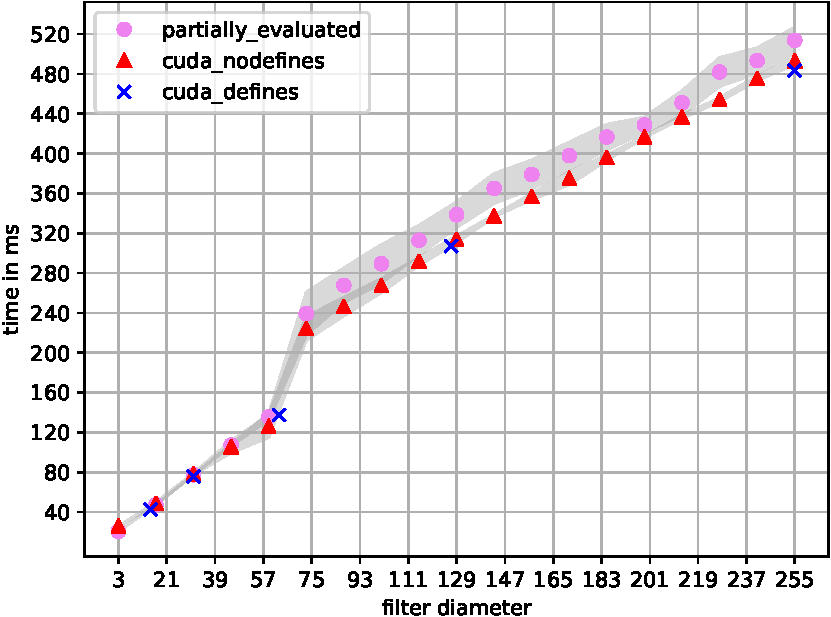
\includegraphics[width=\textwidth]{pictures/Conv_T4-crop}}
\\Results for Tesla T4
\end{center}
\end{minipage}
\end{center}
\end{frame}


\begin{frame}[fragile] \frametitle{Queries Examples}
  \begin{itemize}
  \item Application: image processing
  \item Subject image: random image  of size 1GB %(16384 * 16384)
  \item Filters: random square filters with diameter 3 to 255
  \end{itemize}
  \begin{center}
  \begin{minipage}[t]{0.48\textwidth}
    \begin{center}
  \tikzmark{y}{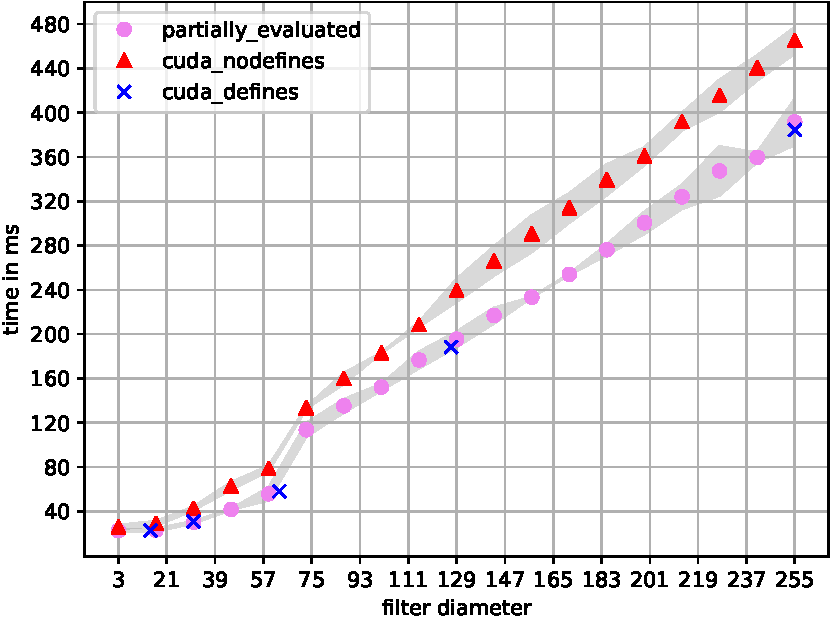
\includegraphics[width=\textwidth]{pictures/Conv_1070-crop}}
  \\Results for GTX-1070
\end{center}
\end{minipage}
\begin{minipage}[t]{0.48\textwidth}
  \begin{center}
{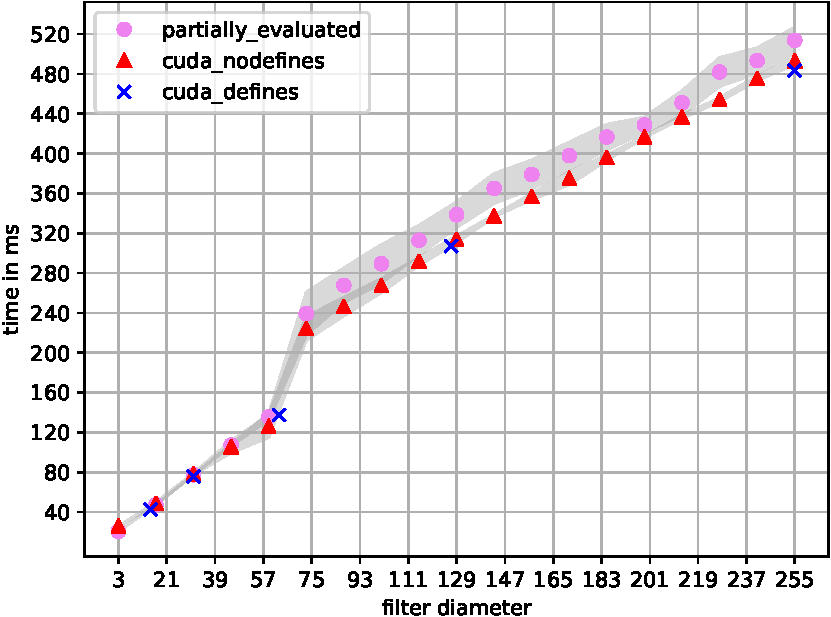
\includegraphics[width=\textwidth]{pictures/Conv_T4-crop}}
\\Results for Tesla T4
\end{center}
\end{minipage}
\end{center}
\end{frame}


\begin{frame}[fragile] \frametitle{Evaluation Setup}

\begin{minipage}[t]{0.51\textwidth}
\vspace{-2cm}
\begin{itemize}
  \item Ubuntu 18.04, Intel Core i7-6700 CPU, 3.4GHz, DDR4 64Gb RAM
  \item Graphs stored in RedisGraph with our extensions
  \item Queries are generated with template for given size of start set
  \item The union of all start sets is a $V$ 
\end{itemize}

\end{minipage}
\begin{minipage}[t]{0.44\textwidth}
{
\rowcolors{2}{black!2}{black!10}
\begin{tabular}{|l|c|c|c|}
\hline
Graph                  & \#V                  & \#E                  & Q     \\
              
\hline
\hline
core                   & 1323                 & 4342                 & $g_1$ \\
pathways               & 6238                 & 18 598               & $g_1$ \\
gohierarchy            & 45 007               & 980 218              & $g_1$ \\
enzyme                 & 48 815               & 109 695              & $g_1$ \\
eclass\_514en          & 239 111              & 523 727              & $g_1$ \\
geospecies             & 450 609              & 2 311 461            & $geo$ \\
go                     & 272 770              & 534 311              & $g_1$ \\
\hline
\end{tabular}
}

\end{minipage}

\vspace{1cm}

\begin{minted}{cypher}
PATH PATTERN S = 
  ()-/ [<:SubClassOf [~S | ()] :SubClassOf] | [<:Type [~S | ()] :Type] /->()
MATCH (src)-/ ~S /->()
WHERE {id_from} <= src.id and src.id <= {id_to}
RETURN count(*)

\end{minted}


\end{frame}

\begin{frame}[fragile] \frametitle{Evaluation Results}  
  \begin{center}
  \begin{minipage}[t]{0.15\textwidth}
  eclass\_514en
  \end{minipage}
  \begin{minipage}[t]{0.4\textwidth}
    \begin{center} 
  \tikzmark{y1}{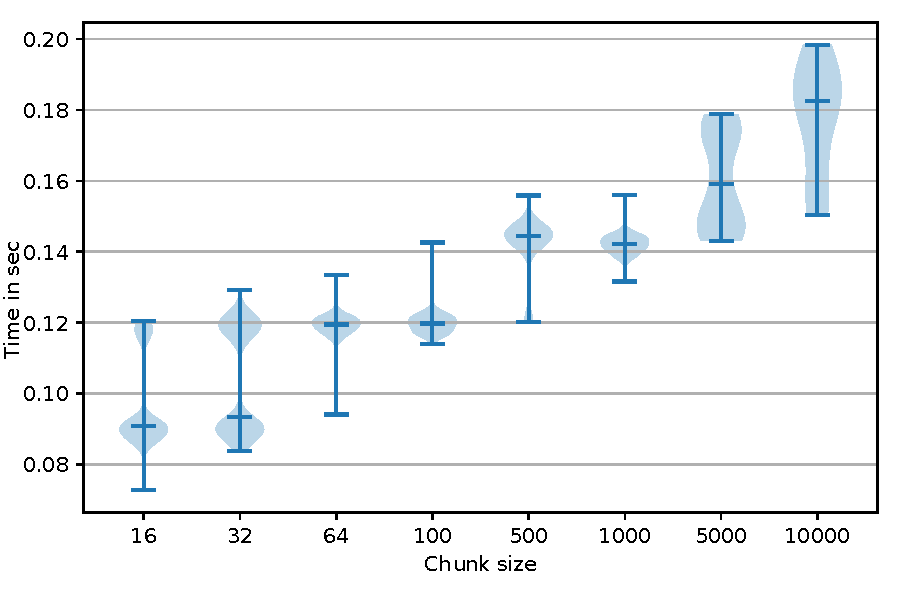
\includegraphics[width=.75\textwidth]{pictures/eclass_514en_time.pdf}}\\
  \tikzmark{y2}{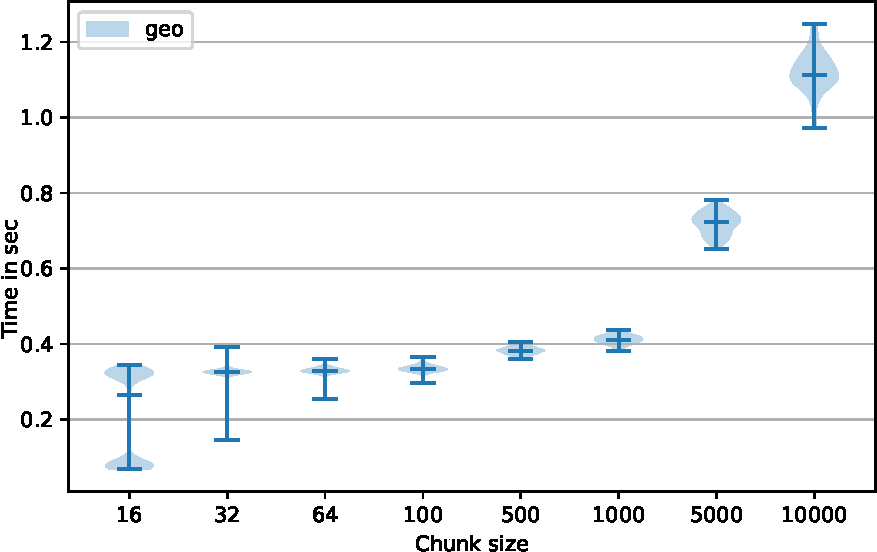
\includegraphics[width=.75\textwidth]{pictures/geospecies_time.pdf}}
\end{center}
\end{minipage}
\begin{minipage}[t]{0.4\textwidth}
  \begin{center}
  \tikzmark{z1}{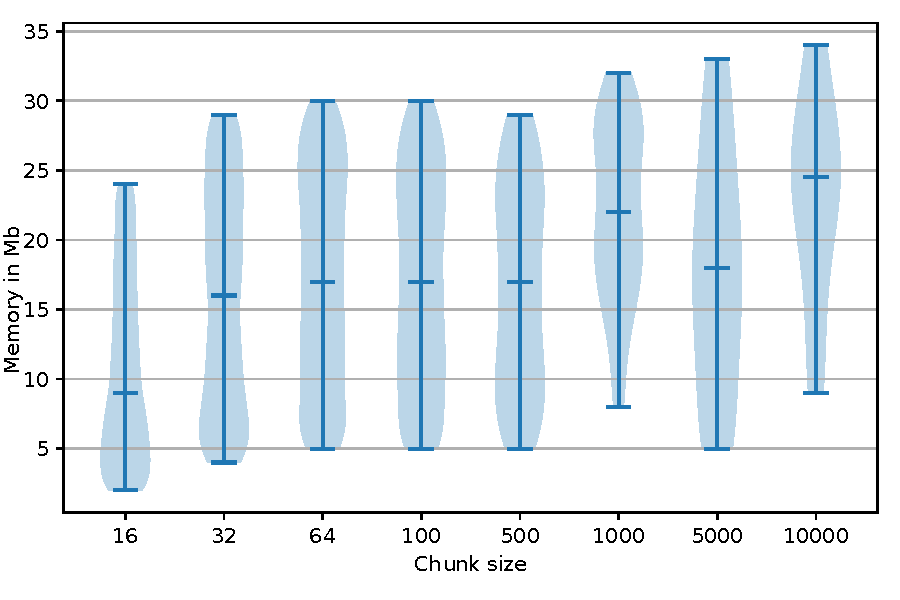
\includegraphics[width=.75\textwidth]{pictures/eclass_514en_mem.pdf}}\\
  \tikzmark{z2}{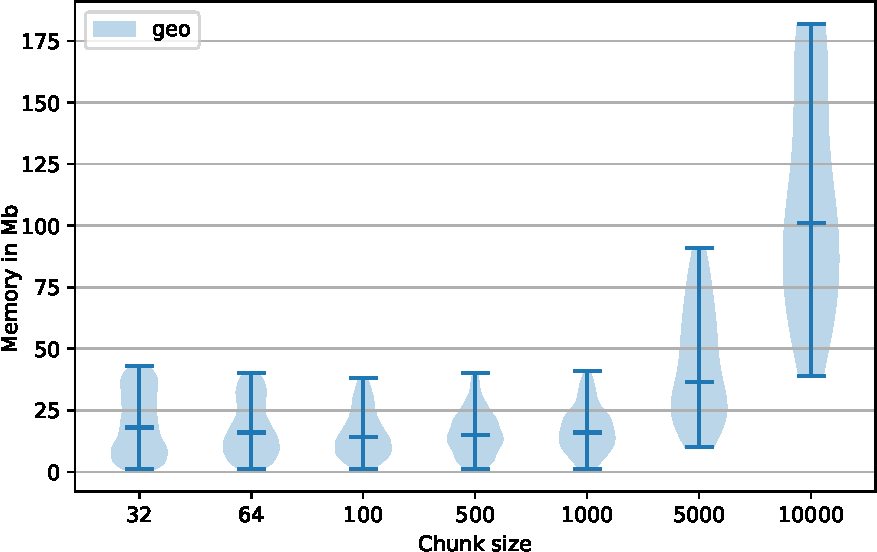
\includegraphics[width=.75\textwidth]{pictures/geospecies_mem.pdf}}
\end{center}
\end{minipage}
\end{center}
\end{frame}


\begin{frame}[fragile] \frametitle{Summary}
  \begin{itemize}
      \item Full-stack support for CFPQ in real-world graph query languages on the top of real-world graph database
      \begin{itemize}
         \item No more ugly context-free grammars
         \item No more custom graph formats and storages
      \end{itemize}
      \item Reasonable performance of context-free path queries
      \begin{itemize}
         \item Multiple-source scenario
         \item Space-time ratio can be tuned
      \end{itemize}
      \item Context-free path queries can be used in applications with well-established tools
  \end{itemize}  
\end{frame}



\begin{frame}[fragile] \frametitle{Future Research}
  \begin{itemize}
    \item Cypher semantics mechanization in Coq
    \begin{itemize}
      \item For new extension
      \item Correctness of translation to linear algebra
    \end{itemize}
    \item Tensor-based CFPQ algorithm
    \begin{itemize}
      \item All paths
      \item Multiple-source
    \end{itemize}
    \item Evaluation
    \begin{itemize}
      \item More data
      \item More algorithms
      \item Scalability of the solution
    \end{itemize}
  \end{itemize}
\end{frame}

\begin{frame}
\frametitle{Contact Information}
\begin{itemize}
  \item Semyon Grigorev:
    \begin{itemize}
      \item \href{mailto:s.v.grigoriev@spbu.ru}{s.v.grigoriev@spbu.ru}
      \item \href{mailto:Semen.Grigorev@jetbrains.com}{Semen.Grigorev@jetbrains.com}
    \end{itemize}

  \item Arseniy Terekhov: \href{mailto:simpletondl@yandex.ru}{simpletondl@yandex.ru}
  \item Vlada Pogozhelskaya: \href{mailto:pogozhelskaya@gmail.com}{pogozhelskaya@gmail.com}
  \item Vadim Abzalov: \href{mailto:vadim.i.abzalov@gmail.com}{vadim.i.abzalov@gmail.com}
  \item Timur Zinnatulin: \href{mailto:teemychteemych@gmail.com}{teemychteemych@gmail.com}

  \vspace{0.5cm}
  \item Try it out (Docker image with all included): \url{!!!}
  \item Sources of RedisGraph extended with CFPQ: \url{!!!}
  \item Sources of Cypher parser extended with path patterns: \url{!!!}
\end{itemize}
\vspace{0.1cm}
\center{\huge{Thanks!}}
\end{frame}
\end{document}
